% Group 9 final report FRAME. Replace every TODO before submission.
% See ../report_plan.md for scope, ownership, evidence and page allocations.
% .latexmkrc resolves IEEEtran from the same supplied template as the survey.
\documentclass[conference]{IEEEtran}

\usepackage{cite}
\usepackage{amsmath,amssymb,amsfonts}
\usepackage{graphicx}
\usepackage{textcomp}
\usepackage[T1]{fontenc}
\usepackage{microtype}
\usepackage{xcolor}
\usepackage{booktabs}
\usepackage{tabularx}
\usepackage[hidelinks]{hyperref}
\usepackage{tikz}
\usetikzlibrary{arrows.meta,positioning}

% Draft helpers: visible owner-labelled placeholders; no invented results.
\newcommand{\placeholder}[2]{%
  \par\noindent
  {\color{blue!65!black}\textbf{TODO (#1):} #2}\par}
\newcommand{\figureplaceholder}[1]{%
  \fbox{\parbox[c][2.5cm][c]{0.92\columnwidth}{%
    \centering\small\textbf{Figure placeholder}\\[0.5em]#1}}}
\newcommand{\unk}{\texttt{<unk>}}
\newcommand{\scoreblank}{\textemdash}

\title{Regional English Accent Robustness in Direct and Cascaded
Speech-to-Text Translation: An Empirical Study}

% Author names and affiliation details follow literature_review/latex/main.tex.
% Nathan coordinates confirmation of these details and the author order.
\author{\IEEEauthorblockN{1\textsuperscript{st} Nathan Naylin}
\IEEEauthorblockA{\textit{Dept. of Science} \\
\textit{University of Auckland}\\
Auckland, New Zealand \\
nhte538@aucklanduni.ac.nz}
\and
\IEEEauthorblockN{2\textsuperscript{nd} Zhitong Li}
\IEEEauthorblockA{\textit{Dept. of Science} \\
\textit{University of Auckland}\\
Auckland, New Zealand \\
zli262@aucklanduni.ac.nz}
\and
\IEEEauthorblockN{3\textsuperscript{rd} Arizona Xing}
\IEEEauthorblockA{\textit{Dept. of Science} \\
\textit{University of Auckland}\\
Auckland, New Zealand \\
lxin541@aucklanduni.ac.nz}
\and
\IEEEauthorblockN{4\textsuperscript{th} Patricia Jennesha}
\IEEEauthorblockA{\textit{Dept. of Science} \\
\textit{University of Auckland}\\
Auckland, New Zealand \\
pjen088@aucklanduni.ac.nz}
\and
\IEEEauthorblockN{5\textsuperscript{th} Jidni Mayukh}
\IEEEauthorblockA{\textit{Dept. of Science} \\
\textit{University of Auckland}\\
Auckland, New Zealand \\
jmay830@aucklanduni.ac.nz}
}

\begin{document}
\maketitle

% OWNER: Nathan; all members verify. Write last. One paragraph, 150--200 words.
\begin{abstract}
\placeholder{Nathan}{Replace with one paragraph covering the problem, frozen
English-to-Chinese seven-accent experiment, three pretrained systems, paired
evaluation and speaker-aware uncertainty, the verified quality ranking, the
limits of the accent-robustness finding, and the main implication. Use results
already established in the body. Avoid citations and unexplained abbreviations.}
\end{abstract}

\begin{IEEEkeywords}
\placeholder{Nathan}{Select concise indexing terms, for example speech
translation, regional English accents, robustness, and paired evaluation.}
\end{IEEEkeywords}

% OWNER: Nathan, organizer. Target: 1--1.5 pages.
\section{Introduction}
\label{sec:introduction}
\placeholder{Nathan}{Introduce the practical importance of reliable
English-to-Chinese speech translation across regional English accents. Establish
the problem using focused external evidence; introduce Direct speech translation,
Cascaded speech translation, automatic speech recognition (ASR) and machine
translation (MT) once.}

\placeholder{Nathan}{State the adopted research question explicitly. Define
accent robustness operationally as between-accent variation in mean sentence
chrF++, while distinguishing overall translation quality. State testable system,
accent, WER-association and MT-variant comparisons. Check historical records
before calling a hypothesis pre-specified; identify exploratory work honestly.}

\placeholder{Nathan}{Explain the matched frozen-input comparison, seven groups
of 600 clips, three systems and paired speaker-aware analysis briefly. End with
actual contributions: the controlled benchmark, uncertainty/accent analysis and
diagnostic/sensitivity evidence. This is an empirical study of pretrained models;
do not claim a new trained model, universal architectural superiority or a causal
accent effect. Introduce the rest of the paper in a short transition.}

% OWNER: Nathan integrates focused inputs from all members. MAXIMUM one page.
\section{Related Work}
\label{sec:related-work}
\placeholder{Nathan + Zhitong}{Write a short synthesis of accent-related ASR
evidence and its limits for downstream translation. Start from the reviewed
accent-codebook study~\cite{prabhu2023accentcodebooks}; cite a source only for
claims it actually supports. Avoid copying the survey's section.}

\placeholder{Nathan + Arizona + Patricia}{Compare Direct and Cascaded ST,
resource/evaluation differences and ASR-to-MT error propagation using the reviewed
context and matched comparison~\cite{sperber2020endtoend,bentivogli2021cascade}.
Explain which aspects the present three-system benchmark tests and which remain
confounded. Add a targeted error-propagation source if the final claim needs it.}

\placeholder{Nathan + Jidni}{Connect accent-labelled speech and translation
references to the chosen evaluation design. Close with the study's specific
position: matched frozen clips, Chinese references, two cascade MT variants,
speaker-aware uncertainty and exploratory diagnostics. Keep this entire section
within one page; do not claim an exhaustive or first-ever gap.}


% OWNER: Nathan. The following method subsections retain their named owners.
\section{Methodology}
\label{sec:methodology}

The experiment proceeds from a frozen dataset to matched system outputs,
translation scoring and paired statistical comparisons. Small pilots check
engineering feasibility before the three pretrained systems process the same
inputs without parameter fitting. Predictions are aligned by clip to compare
system quality, accent variation and ASR associations. Exploratory marker
diagnostics and subset checks then examine output behaviour and the stability
of the comparison. The implementation is available on
GitHub.\footnote{\url{https://github.com/Nlhmmh/cs760-accent-st-robustness-ml-research}}
The repository includes the de-identified frozen evaluation metadata, pilot
metadata, archived predictions, run records and analysis code. The evaluation
CSV contains the source transcripts, accent labels, pseudonymous speaker IDs
and Chinese references. Recordings are not included in the repository;
repeating inference requires obtaining the matching audio while preserving
the frozen metadata and row order. Scoring and statistical analysis can use the
archived predictions without loading speech models or audio. The subsections
below describe the data, inference controls, evaluation, statistics and
diagnostic designs in that order.

% OWNER: Arizona. Target: about 0.75 page including the dataset table.
\subsection{Evaluation Data and Reference Construction}
\label{sec:data}
\placeholder{Arizona}{Describe Common Voice Scripted Speech 26.0 English
and CoVoST 2 Simplified Chinese references, with source
citations~\cite{ardila2020commonvoice,wang2021covost2}. Specify the actual release
separately from the original Common Voice paper. Explain first self-reported
accent selection, normalized-sentence matching, first-reference retention and
reference spot-checks without inventing human validation.}

\placeholder{Arizona}{State duration/plausibility filters, their actual
thresholds and origin in the five-group pool; the later two-group addition;
100-clip speaker cap; seed 760 and 600 clips per group. Report total speakers,
repeated speakers/sentences and duration coverage. Define pseudonymous speaker
sample ID separately from the generated unique clip ID. Explain label granularity,
content imbalance, reference matching and de-identification limitations.}

\begin{table}[t]
\caption{Evaluation-set composition. TODO (Arizona): fill verified counts,
define every column and explain pooled regional labels in the text.}
\label{tab:dataset}
\centering
\small
\begin{tabularx}{\columnwidth}{@{}Xrr@{}}
\toprule
Accent group & Clips & Speakers \\
\midrule
England English & \scoreblank & \scoreblank \\
Filipino & \scoreblank & \scoreblank \\
Hong Kong English & \scoreblank & \scoreblank \\
India and South Asia & \scoreblank & \scoreblank \\
Malaysian English & \scoreblank & \scoreblank \\
Southern African & \scoreblank & \scoreblank \\
United States English & \scoreblank & \scoreblank \\
\midrule
Total & \scoreblank & \scoreblank \\
\bottomrule
\end{tabularx}
\end{table}

% OWNER: Nathan. Target: about 0.75 page including diagram/configuration.
\subsection{Systems and Controlled Inference}
\label{sec:systems}
\placeholder{Nathan}{Describe SeamlessM4T v2-large Direct ST and Whisper
large-v2 followed by NLLB-600M or NLLB-3.3B. Cite the v2 context, Whisper and
NLLB sources~\cite{seamless2023,radford2023whisper,nllb2022}. Give exact checkpoint
IDs/resolved revisions and target/source language codes. Explain that model
families, training resources and objectives differ.}

\placeholder{Nathan}{Specify mono 16 kHz audio, actual fixed greedy settings,
seed, FP16/T4 environment and relevant library versions from run records.
Explain staged ASR then MT and no reference transcripts supplied to MT. Describe
pilots as engineering checks, checkpointing, successful-run/limit checks, ID and
fingerprint alignment, and matching archived ASR strings from separate runs.
If runtime is reported, distinguish Direct pipeline time, Cascade stage-sum time,
and wall-clock time; loading/warm-up are excluded from recorded sample timings.}

\begin{figure}[t]
\centering
\figureplaceholder{Nathan: matched English speech, Direct ST, Whisper followed
by both NLLB variants, and common Chinese reference evaluation.}
\caption{System comparison. TODO (Nathan): replace with an original or properly
credited diagram; adapt the survey diagram to the completed three-system design.}
\label{fig:systems}
\end{figure}

% Optional compact table: include essential settings in prose if a table is wider
% or less readable. Keep full model revisions in the paper if needed for replay.

% OWNER: Patricia. Target: about 0.5 page.
\subsection{Evaluation Metrics}
\label{sec:metrics}



Translations are scored with SacreBLEU 2.6.0 against the single CoVoST~2
Chinese reference for each clip. \emph{Corpus BLEU} [9] pools n-gram
counts (up to 4-grams) over all clips and applies a brevity penalty. We
use SacreBLEU's Chinese tokenizer (\texttt{tokenize=zh}), which splits
Chinese into characters. The default 13a tokenizer separates punctuation
but does not segment Chinese characters, and the tokenizer must be
reported with BLEU scores [12]. \emph{chrF} [10] is
an F-score over character n-grams (order 6, $\beta=2$, whitespace
excluded by default). \emph{chrF++} [11] adds word unigrams and bigrams to
chrF (word order 2). chrF++ does not use BLEU's Chinese tokenizer. Its
word component is extracted by splitting on whitespace with some
punctuation handling, so an unspaced Chinese sentence forms very few
words. In this evaluation chrF++ is lower than chrF for every system.
The two are different metric definitions, so their values are not
interchangeable quality scales. Scores are on a 0--100 scale, and higher
is better.
 
We report two kinds of chrF++. \emph{Corpus} scores pool statistics over
a set of clips and describe overall quality. \emph{Mean sentence chrF++}
averages the score of each clip and is the quantity used for paired
statistics and accent comparisons, because each clip then has its own
score. The two are not interchangeable.
 
\emph{Word error rate} (WER) diagnoses the cascade's ASR stage only. It
compares the Whisper transcript with the Common Voice sentence as
$(S+D+I)/N$ for substitutions, deletions, insertions and $N$ reference
words. We use \emph{normalized} WER, after lowercasing, removing
punctuation, collapsing repeated spaces and stripping the ends. Raw WER is
10.56\%, and normalization lowers it to 5.97\%, because many raw errors
are formatting differences such as ``Mr'' and ``Mr.''. \emph{Pooled}
corpus WER divides total errors by total words, while \emph{mean per-clip}
WER averages the clip values. Direct ST exposes no transcript, so it has
no WER. Finally, a \emph{literal marker} is an output containing the exact
string \texttt{<unk>}, counted separately from the tokenizer's special
unknown-token ID.
 
\emph{Reproducibility.} Following Post [12], the SacreBLEU 2.6.0
signatures are as follows. BLEU:
\texttt{nrefs:1\allowbreak|case:mixed\allowbreak|eff:no\allowbreak|tok:zh\allowbreak|smooth:exp\allowbreak|version:2.6.0}.
chrF:
\texttt{nrefs:1\allowbreak|case:mixed\allowbreak|eff:yes\allowbreak|nc:6\allowbreak|nw:0\allowbreak|space:no\allowbreak|version:2.6.0}.
chrF++ differs only in \texttt{nw:2}. Mean sentence chrF++ uses the same
chrF++ settings. The signatures were printed after the full runs, using
the same scorer settings as the reported scores.
% OWNER: Zhitong. Target: about 0.5 page; type relevant equations here.
\subsection{Statistical Analysis}
\label{sec:statistics}
\placeholder{Zhitong}{Define paired mean sentence chrF++ gaps and each system's
max-minus-min accent-mean spread in typed equations. Introduce notation once:
clip, accent, system, sentence score, mean and paired difference. Explain the
1,000-resample, seed-760, accent-stratified speaker-cluster bootstrap, shared
resamples across systems and 95\% percentile intervals, with appropriate paired
evaluation context~\cite{koehn2004significance}. Cite additional statistical
sources if required for methods not supported by this paper.}

\placeholder{Zhitong}{Describe clip-resampling sensitivity, speaker-mean versus
clip-level rank tests, Kruskal--Wallis, Dunn comparisons with Holm correction
within each accent-pair family, paired Wilcoxon tests and effect sizes. Explain
Spearman WER associations: clip-level observations with clustered uncertainty.
State clip-weighted estimands and unmodelled repeated-content dependence;
identify exploratory tests and the correction scope.}

% Insert real equations, for example the paired mean gap and accent spread,
% after choosing consistent notation. No fabricated statistical definitions.

% OWNER: Nathan. Post-hoc experiments; official predictions are preserved.
\subsection{Earlier Direct-Output Diagnostics}
\label{sec:earlier-diagnostic-method}

We first audited the frozen Direct outputs for the exact string \unk{}, its
frequency by accent and repeated sentence, runtime/generation flags, and the
pinned tokenizer's encoding of Chinese references. Reference-tokenizer
co-occurrence is descriptive and does not identify which token the model
generated. We therefore selected five originally affected clips per accent
using seed 760, giving 35 clips, and reran the same Direct checkpoint while
retaining generated token IDs. This sensitivity experiment used CPU FP32,
PyTorch/torchaudio 2.8.0 and Transformers 4.57.6, rather than the full run's
GPU FP16 environment.

We compared greedy decoding, greedy decoding with special UNK ID~1 suppressed,
beam search with five beams, and beam search with that ID suppressed. Sampling
remained disabled and the 256-new-token limit was retained. A second check on
the same selected clips blocked the ordinary token sequences that spelled the
visible marker, using \texttt{bad\_words\_ids}. Each experiment checked baseline
agreement with the archived translations, counted literal markers and special
UNK IDs separately, and scored the same subset using SacreBLEU 2.6.0. Changed
outputs were inspected for alternative marker spellings. These post-hoc
experiments did not alter the official 4,200 predictions.

% OWNER: Arizona. Share the diagnostic/sensitivity page allocation.
\subsubsection{Accent association}
\label{sec:further-diagnostic-method}

A failure mode specific to one system could distort the accent comparison if
it varied across groups. Complementing the decoding checks, the following
analyses examine whether the literal \unk{} marker is linked to accent,
input modality or source wording (Table~\ref{tab:further-diagnostics}).
Checks that re-ran the model used the
Direct checkpoint, revision and decoding controls of Section~\ref{sec:systems}
on a Colab T4 GPU in FP16; exact library versions were not recorded. The
case-insensitive pattern \verb|<\s*unk\s*>| selects the same 508 archived
clips as exact-string matching. In all regressions, sentence length counts
whitespace-delimited words and sentence clusters use the original English
strings.

Logistic regressions of marker presence on accent, with and
without sentence length, tested the six accent coefficients (United States
English as reference) jointly by Wald tests, once with speaker-clustered and
once with sentence-clustered standard errors.

\subsubsection{Input modality}
The same checkpoint translated each clip's reference transcript
and Whisper transcript in batches of 32
(\texttt{SeamlessM4Tv2ForTextToText}). A speech re-run of 700
clips, randomly sampled with 100 per accent group (seed 760), kept the
generated token IDs to count special UNK ID~1, which decoding removes.

\subsubsection{Source wording}
Sentence-clustered logistic regressions related marker
presence to sentence length, proper-noun presence and the minimum
general-English Zipf frequency~\cite{speer2022wordfreq} of the clip's content
lemmas, the lower-cased dictionary forms of alphabetic tokens tagged NOUN,
VERB, ADJ or ADV (PROPN excluded) by spaCy
\texttt{en\_core\_web\_sm}~\cite{honnibal2020spacy}. The 48 clips without a
content token were assigned the median observed clip-level minimum (4.12).
Word removal used the 439 distinct English sentences of the 508 speech-marked
clips, restricted to the 385 whose text-input translation reproduced the
marker. At the decoding step where the first marker began, each whitespace-delimited
input word was deleted in turn, with the already generated output tokens
fixed. The selected word was the one whose deletion most reduced the summed
probability of the two alternative next tokens that begin the marker. Each sentence was
then translated afresh, without the fixed prefix, once without the selected
word and, as a control, once without another word chosen at random (seed
760). The outcome is the proportion of the 385 sentences whose new
translation contains no marker, with Wilson intervals. The Wilson intervals
treat clips in the special-ID check and sentences in word removal as
independent units.

% OWNER: Jidni. Share the diagnostic/sensitivity page allocation.
\subsection{Subset and Speaker Sensitivity Checks}
\label{sec:sensitivity-method}
\placeholder{Jidni}{Specify common marker-free subset selection for all
systems, zero/positive-WER subsets, one-clip-per-speaker sampling and its seed,
and the post-hoc Cascade-3.3B fallback rule. State estimands and uncertainty
settings. If examples are used, define the worst-ten-per-accent/system selection
and how the team checked their interpretation. Do not describe subset selection
or changed outputs as a validated remedy.}


% OWNER: Nathan. Member-owned results subsections follow unchanged.
\section{Experiments and Results}
\label{sec:results}

All three full inference runs completed successfully for 4,200 clips, with no
recorded inference failures or generation-limit flags. The following results
first compare overall and accent-level translation quality, then examine
paired uncertainty and accent variation. Direct-output diagnostics and subset
sensitivity checks are reported separately from the frozen benchmark so that
their selected samples and changed decoding settings remain explicit.

% OWNER: Patricia. Target: about 1 page including the overall table.
\subsection{Overall and Per-Accent Translation Quality}
\label{sec:quality-results}
\placeholder{Patricia}{Fill Table~\ref{tab:overall-quality} from the archived
three-system evidence and explain ranking and magnitudes. Report corpus WER
and mean per-clip WER separately. Summarize per-accent corpus BLEU/chrF++ and
sentence means with a compact table or by referring to the shared accent figure.
Discuss meaning for the RQ rather than only listing scores. Leave uncertainty
and test interpretation to Section~\ref{sec:statistical-results}.}

\begin{table}[t]
\caption{Overall translation quality. TODO (Patricia): fill the first three
columns with corpus scores and the last with mean sentence chrF++; higher is better.}
\label{tab:overall-quality}
\centering
\small
\begin{tabular}{@{}lrrrr@{}}
\toprule
System & BLEU & chrF & chrF++ & Sent. mean \\
\midrule
Direct & \scoreblank & \scoreblank & \scoreblank & \scoreblank \\
Cascade-600M & \scoreblank & \scoreblank & \scoreblank & \scoreblank \\
Cascade-3.3B & \scoreblank & \scoreblank & \scoreblank & \scoreblank \\
\bottomrule
\end{tabular}
\end{table}

% Integrated from research_report/member_4/zhitong_sections.tex.
\subsection{Uncertainty and Accent Variation}
\label{sec:statistical-results}

Paired comparisons assess whether the quality ranking is supported after
accounting for speaker dependence. Separate analyses examine the spread of
accent means and whether the size of each system gap varies across accents.

\begin{table}[t]
\caption{Paired mean sentence chrF++ gaps (points) with speaker-clustered 95\% intervals. Positive gaps favour the first-named system.}
\label{tab:paired-gaps}
\centering
\small
\begin{tabular}{lcc}
\toprule
Comparison & Mean gap & 95\% CI \\
\midrule
Direct $-$ Cascade-600M & $+7.00$ & [6.45, 7.60] \\
Direct $-$ Cascade-3.3B & $+4.99$ & [4.39, 5.70] \\
Cascade-3.3B $-$ Cascade-600M & $+2.01$ & [1.61, 2.42] \\
\bottomrule
\end{tabular}
\end{table}

\begin{table}[t]
\caption{Mean sentence chrF++ by accent and Direct-minus-Cascade gaps with speaker-clustered 95\% intervals (unadjusted for multiplicity). Eng, Fil, HK, Ind, Mal, SAf, US = England, Filipino, Hong Kong, India and South Asia, Malaysian, Southern African, United States; $n_{\mathrm{spk}}$ = speakers; D, C6, C3 = Direct, Cascade-600M, Cascade-3.3B.}
\label{tab:accent-gaps}
\centering
\footnotesize
\setlength{\tabcolsep}{3pt}
\begin{tabular}{lrcccrr}
\toprule
Accent & $n_{\mathrm{spk}}$ & D & C6 & C3 & D$-$C6 & D$-$C3 \\
\midrule
Eng & 398 & 27.9 & 22.5 & 23.6 & 5.4 [4.3, 6.5] & 4.2 [3.1, 5.3] \\
Fil & 72 & 28.9 & 21.2 & 24.5 & 7.7 [6.2, 9.3] & 4.4 [3.2, 5.8] \\
HK & 41 & 28.3 & 20.0 & 21.3 & 8.4 [6.1, 10.2] & 7.0 [4.6, 9.7] \\
Ind & 356 & 27.4 & 19.8 & 22.0 & 7.6 [6.5, 8.9] & 5.4 [4.3, 6.7] \\
Mal & 61 & 28.0 & 20.2 & 22.4 & 7.9 [6.5, 9.3] & 5.7 [4.5, 7.0] \\
SAf & 131 & 27.2 & 21.7 & 23.7 & 5.5 [4.3, 6.7] & 3.5 [2.5, 4.6] \\
US & 527 & 27.3 & 20.7 & 22.6 & 6.6 [5.4, 7.8] & 4.7 [3.6, 5.8] \\
\bottomrule
\end{tabular}
\end{table}

\subsubsection{System gaps}
All three overall gap intervals exclude zero (Table~\ref{tab:paired-gaps}),
supporting Hypotheses~\ref{hyp:quality} and~\ref{hyp:mt-size}.
Cascade-3.3B gains about two points over Cascade-600M.
Within every accent the
Direct-minus-Cascade intervals also exclude zero (Table~\ref{tab:accent-gaps}),
and the speaker-level matched-pairs rank-biserial correlations are positive
throughout (0.53--0.93 against Cascade-600M; 0.39--0.91 against Cascade-3.3B).

The Cascade-3.3B lift is positive in all seven accents. Its mean-gap bootstrap
intervals remain above zero for England English (0.18 to 2.19) and Hong Kong
English (0.09 to 2.52), whereas the speaker-level Wilcoxon tests give
$p=0.138$ and $0.089$. These procedures assess different quantities: the
bootstrap estimates the clip-weighted mean gap, while the rank test uses
speaker-mean paired differences. The two summaries therefore need not agree.

\subsubsection{Accent means and spread}
\begin{figure}[t]
\centering
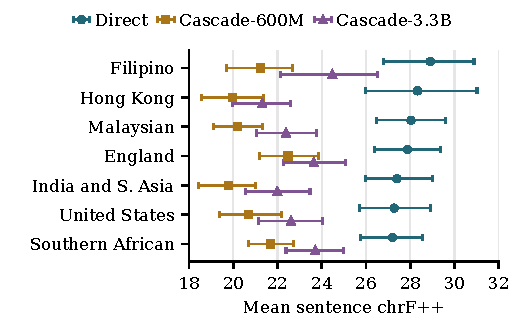
\includegraphics[width=\columnwidth]{figures/accent_means.pdf}
\caption{Mean sentence chrF++ with unadjusted 95\% speaker-clustered
bootstrap intervals. Overlap alone does not test robustness differences.}
\label{fig:accent-means}
\end{figure}

Direct has the smallest observed between-accent spread, but the differences
between systems remain uncertain (Fig.~\ref{fig:accent-means}).
The spread $R_s$ is 1.71 [1.4, 5.1] points
for Direct, 2.70 [2.0, 4.7] for Cascade-600M and 3.17 [2.0, 5.7] for
Cascade-3.3B. These intervals are right-skewed because a maximum minus a minimum
of noisy means is biased upward. All three differences in spread have
intervals that include zero (e.g.\ $-1.0$ [$-2.3$, 2.3] for
Direct $-$ Cascade-600M). Higher translation scores therefore do not establish
stronger accent robustness under the study's spread-based definition;
Hypothesis~\ref{hyp:spread} remains unresolved.

A speaker-level Kruskal--Wallis test detects accent differences only for
Cascade-600M ($p=0.041$, $\epsilon^2=0.008$; Direct $p=0.185$,
Cascade-3.3B $p=0.168$), a single uncorrected result. The cascades largely agree
in their accent orderings (Spearman $\rho=0.82$), whereas Direct follows neither
($\rho=-0.18$ and $-0.07$; seven means only). Hong Kong English ranks second
for Direct but sixth or seventh for the cascades, and its intervals are wide
because it has only 41 speakers.

\subsubsection{Variation in system gaps across accents}
\label{sec:statistical-accent-gap-variation}
The Direct-minus-Cascade gap varies across accents, with small speaker-level
effects against Cascade-600M ($H(6)=21.4$, $p=0.0015$, $\epsilon^2=0.014$)
and Cascade-3.3B ($H(6)=17.2$, $p=0.009$, $\epsilon^2=0.011$); clip-level
tests agree. Against Cascade-600M the gap is largest for Hong Kong English
(8.4) and smallest for England English (5.4); against Cascade-3.3B it is
largest for Hong Kong English (7.0) and smallest for Southern African
speakers (3.5).

Few individual accent pairs differ after correction: 2 of 21 against
Cascade-600M and 1 of 21 against Cascade-3.3B, all with small effects
(Cliff's $|\delta|\le 0.30$). Malaysian versus United States English is the
pair common to both. Clip-level tests flag different pairs, so pair-level
conclusions are fragile. Direct's flatter accent means suggest that the
variation comes mostly from the cascades, but the uncertain spread differences
prevent a firm conclusion. The Cascade-3.3B lift shows no detectable variation
across accents ($p=0.168$ speaker level); this does not establish equal gains.

\subsection{Recognition Errors and Translation Scores}
\label{sec:statistical-asr-associations}
The accent-level WER pattern in Table~\ref{tab:accent} motivates a clip-level
analysis of recognition and translation scores. Higher normalized WER is
associated with lower cascade scores ($\rho=-0.19$ [$-0.22$, $-0.16$] for
Cascade-600M; $-0.20$ [$-0.23$, $-0.17$] for Cascade-3.3B) and with a larger
Direct advantage ($\rho=0.13$ [0.10, 0.16] and $0.17$ [0.14, 0.20]). All
intervals exclude zero, overall and within each accent, supporting
Hypothesis~\ref{hyp:wer}. The associations are weak and observational;
they do not identify ASR error as the cause.

These associations describe the cascade's exposed recognition stage. The
following diagnostics examine a separate feature of Direct outputs: the
visible \unk{} marker. Section~\ref{sec:synthesis-results} then compares
system gaps within WER-defined subsets.

% OWNER: Nathan. Target: about 0.35 page.
\subsection{Literal Markers and Earlier Decoding Checks}
\label{sec:earlier-diagnostic-results}
\placeholder{Nathan}{Report frozen-run visible-marker counts/rates and the
35-clip decoding/constraint findings with exact denominators. Distinguish literal
\unk{} from special UNK IDs; report baseline reproduction and changed-output
quality. Explain why the tested constraints did not establish a validated fix.
Do not generalize small-subset scores to all 4,200 clips.}

% OWNER: Arizona. Target: about 0.65 page; select findings, do not copy all extras.
\subsubsection{Accent association}

\begin{table}[t]
\caption{Accent, input-modality and source-wording diagnostics for Direct. All checks are
post hoc and leave the archived predictions unchanged. Intervals are 95\%:
sentence-clustered regression (word frequency) and Wilson (special ID, word
removal).}
\label{tab:further-diagnostics}
\centering
\footnotesize
\begin{tabularx}{\columnwidth}{@{}>{\raggedright\arraybackslash}p{1.25cm}
  >{\raggedright\arraybackslash}p{2.05cm}>{\raggedright\arraybackslash}X@{}}
\toprule
Check & Input; sample & Finding \\
\midrule
Accent & Archived output; 4,200 clips &
  Joint accent test $\chi^2(6)=5.34$, $p=0.50$ \\
\addlinespace[2pt]
Text input & Reference transcript; 4,200 clips &
  449 of 508 speech-marked clips marked again (88.4\%) \\
\addlinespace[2pt]
Special ID & Speech, token IDs kept; 700 clips &
  ID~1 in 74 clips (10.6\% [8.5, 13.1]); none has the marker \\
\addlinespace[2pt]
Word frequency & Archived output; 4,200 clips &
  OR 0.52 [0.48, 0.57] per Zipf unit of the rarest content lemma,
  length-adjusted \\
\addlinespace[2pt]
Word removal & Reference transcript; 385 sentences &
  Re-translation without the marker in 310 (80.5\% [76.3, 84.2]) after
  selected-word vs.\ 38 (9.9\% [7.3, 13.3]) after random-word deletion \\
\bottomrule
\end{tabularx}
\end{table}

The group marker rates reported above span about three percentage
points, and the speaker-clustered joint test did not detect an association
between accent and marker presence (Table~\ref{tab:further-diagnostics});
sentence clustering or length adjustment does not change this ($p=0.45$ and
$0.48$, respectively). Of the 370 normalized sentences recorded more than
once, six were marked in some recordings but not others.

\subsubsection{Input modality}
\label{sec:further-diagnostic-results}
With reference-transcript input, the marker recurs in most speech-marked
clips and appears in only 79 of the 3,692 speech-unmarked clips (2.1\%), so
the anomaly is not exclusive to speech input. Whisper-transcript input gives
a similar overall rate (11.9\%, versus 12.6\% with reference transcripts).
Marker status differs between speech and reference-transcript input for 138
clips (59 marked only with speech input, 79 only with reference-transcript
input). In the
700-clip speech re-run, 694 outputs reproduced their archived strings exactly,
and none of the 74 clips with special UNK ID~1 showed the visible marker in
either run. Outputs with hidden ID~1 can therefore remain in the marker-free
subset of Section~\ref{sec:synthesis-results}.

\subsubsection{Source wording}
Marker presence is associated with source vocabulary
that is rare in general English. The rate falls from 31.3\% (82 of 262 clips)
when the rarest content lemma has Zipf $\le 2.5$ to 5.1\% (119 of 2,323) when
it exceeds 4 (including imputed clips). After length adjustment, each
tenfold increase in that lemma's frequency is associated with about half the
odds of a marker (Table~\ref{tab:further-diagnostics}). Proper nouns show no
clear association (OR 0.95 [0.75, 1.21], adjusted for length and rarest-lemma
frequency). Among the 385 sentences with marked text-input translations,
re-translation without the selected word was marker-free for 80.5\% of them,
against 9.9\% without a random other word
(Table~\ref{tab:further-diagnostics}). The gap remains in the 161 sentences
whose random word is not a spaCy stop word (78.3\% versus 13.0\%). Selected words are rarer than the other non-stop words
(median surface-form Zipf 3.8 versus 4.6). Because each was chosen to
maximize the drop in summed marker-start probability at one decoding step,
the deletion comparison measures sensitivity to the targeted deletion and
does not isolate a causal effect of word rarity.

Marker occurrence is associated with rarer source wording, while no
association with accent was detected; its internal cause remains unresolved. The text-input and token-ID checks also show that
neither speech input nor generation of special UNK ID~1 is required for the
visible marker to occur. The word-removal experiment measures marker
presence rather than translation quality. Section~\ref{sec:synthesis-results} examines whether
the system ranking persists after visibly marked clips are excluded.

% Integrated from research_report/member_5/jidni_part.md.
\subsection{Sensitivity Checks and Larger-MT Interpretation}
\label{sec:synthesis-results}

Table~\ref{tab:sensitivity} lists the checks of Section~\ref{sec:sensitivity-method}.

\begin{table}[t]
\caption{Selected sensitivity checks. Gaps are mean sentence chrF++ (points) with 95\% intervals, speaker-clustered unless stated. D, C6, C3 = Direct, Cascade-600M, Cascade-3.3B.}
\label{tab:sensitivity}
\centering
\footnotesize
\setlength{\tabcolsep}{3pt}
\begin{tabularx}{\columnwidth}{@{}>{\raggedright\arraybackslash}p{0.25\columnwidth}
  >{\raggedright\arraybackslash}p{0.18\columnwidth}
  >{\raggedright\arraybackslash}X@{}}
\toprule
Check & Clips & Statistic / finding \\
\midrule
Common marker-free subset & 3,692 &
  D $-$ C3 $+5.42$ [4.75, 6.08];\newline
  D $-$ C6 $+7.50$ [6.88, 8.11] \\
\addlinespace[2pt]
Normalized $\mathrm{WER}=0$ & 2,952 &
  D $-$ C3 $+3.61$ [3.04, 4.24];\newline
  C3 $-$ C6 $+2.27$ [1.76, 2.76] \\
\addlinespace[2pt]
Normalized $\mathrm{WER}>0$ & 1,248 &
  D $-$ C3 $+8.24$ [7.38, 9.17];\newline
  C3 $-$ C6 $+1.40$ [0.90, 1.92] \\
\addlinespace[2pt]
One clip per speaker & 1,586 &
  D $-$ C3 $+4.69$ [3.94, 5.51] (clip bootstrap) \\
\addlinespace[2pt]
C3 fallback on marked outputs & 4,200 (508 replaced) &
  Corpus chrF++ $25.08 \rightarrow 24.89$; BLEU $38.86 \rightarrow 38.54$ \\
\bottomrule
\end{tabularx}
\end{table}

\subsubsection{Marker-free subset}
On the 3,692 unmarked clips Direct's corpus chrF++ rises from 25.08 to 26.32. Both cascades rise as well, Cascade-3.3B from 20.06 to 20.77 and Cascade-600M from 18.44 to 19.10, so every system scores lower on the marked clips. The paired gaps on the unmarked clips are +5.42 [4.75, 6.08] against Cascade-3.3B and +7.50 [6.88, 8.11] against Cascade-600M, slightly above the full-set values in Table~\ref{tab:paired-gaps}, and each per-accent Direct-minus-Cascade interval stays above zero. On the 508 marked clips alone Direct also scores above both cascades (corpus chrF++ 17.55 against 15.46 and 14.22). The quality ranking holds with the marked outputs removed. The two groups of clips contain different sentences, so the 1.24-point rise in Direct's corpus chrF++ mixes the marker with sentence difficulty, and cannot be interpreted as the marker's effect.

\subsubsection{WER subsets}
Where Whisper's transcript matches the reference, which covers 70.3\% of clips, Direct leads Cascade-3.3B by +3.61 [3.04, 4.24]. Where the transcript contains at least one error the lead is +8.24 [7.38, 9.17]. Error clips make up 22.8\% of United States English and 36.2\% of Malaysian English, the groups with the smallest and one of the largest Direct-minus-Cascade-600M gaps in Table~\ref{tab:accent-gaps}. Recognition errors that reach the MT stage would produce this pattern, and the Spearman associations of Section~\ref{sec:statistical-asr-associations} point the same way. The split uses the cascade's own output as its dividing line. Direct's lead on error-free transcripts shows that the systems differ in more than recognition.

\subsubsection{Larger MT}
Cascade-3.3B improves on Cascade-600M in every accent group (Table~\ref{tab:accent-gaps}), with no detectable variation across groups (Section~\ref{sec:statistical-accent-gap-variation}). On error-free transcripts the lift is +2.27 [1.76, 2.76]; on clips with recognition errors it is +1.40 [0.90, 1.92]. For these checkpoints the larger MT model gained less where the transcript was wrong. The larger model narrows the gap to Direct and leaves most of it in place. A comparison that varies MT capacity alone cannot show what a larger or differently trained MT model would do.

\subsubsection{Speaker dependence}
With one clip per speaker the gaps are +6.19 [5.37, 6.90] against Cascade-600M, +4.69 [3.94, 5.51] against Cascade-3.3B and +1.50 [0.91, 2.16] between the cascades. These agree with the speaker-clustered estimates on the full set.

\subsubsection{Fallback}
Replacing Direct's output with the Cascade-3.3B translation on the 508 marked clips lowers corpus chrF++ from 25.08 to 24.89 and corpus BLEU from 38.86 to 38.54. On these clips the marked Direct outputs score above the cascade's translations, so the substitution did not improve scores.

\subsubsection{Worst clips}
In five of the seven groups, at least half of Direct's ten lowest-scoring clips score exactly zero. The cascades' worst clips in India and South Asia and in Hong Kong English carry mean WER between 0.31 and 0.56, against 0.06 over the whole set. Direct's worst clips carry mean WER of about 0.1, and 14\% of them contain the marker, near the 12.1\% base rate. Several references are non-literal. The reference for "There you have it!" is \begin{CJK*}{UTF8}{gbsn}给你！\end{CJK*}, and the literal \begin{CJK*}{UTF8}{gbsn}这就是它!\end{CJK*} scores zero against it. A low automatic score on such a clip measures reference matching and identifies no system error.

\subsubsection{What the checks show}
The quality ranking survives every check. Removing the marked outputs or counting each speaker once leaves Direct ahead of both cascades with the cascade ordering unchanged, and the same holds within each WER subset. The accent findings come out qualified. The gap's association with recognition errors fits the accent pattern in Table~\ref{tab:accent-gaps}, yet the subsets are defined by outcomes and by content, so they cannot attribute the gap to accent handling or to architecture, and Direct's lead on error-free transcripts stays unexplained.


% OWNER: Nathan integrates evidence and limitations supplied by every member.
% Target: about 0.75 page. This is counted inside the 12-page main-body limit.
\section{Discussion and Limitations}
\label{sec:discussion}
\placeholder{Nathan + all}{Connect the system-quality, accent-variation,
ASR-association, MT-variant and marker findings into one answer to the main RQ.
Explain the distinction between a positive system gap and stronger robustness
under the chosen spread measure. Discuss plausible explanations only at the
strength allowed by this design and the external literature.}

\placeholder{Nathan + all}{Synthesize limitations: one language direction and
specific pretrained checkpoints; model/training/capacity confounds; self-reported
pooled accent labels; unequal speaker/content/recording distributions; repeated
sentences not jointly modelled with speakers; single-reference automatic metrics
without human-quality validation; exploratory tests/correction scope; text-only
and selected-subset diagnostic limits; private data and incomplete environment/
supplementary replay records. State the practical consequences, not only a list.}

% OWNER: Nathan integrates all members' future-work inputs. About one page.
\section{Conclusion and Future Work}
\label{sec:conclusion}
\placeholder{Nathan}{Give a high-level summary of the problem, matched
three-system experiment and supported answers. State the frozen-set quality
ranking, what is known about accent variation, and what remains inconclusive
about relative robustness. Refer to established results rather than introduce
new numbers, tests or causal claims.}

\placeholder{Nathan + all}{Prioritize feasible future research for a master's
project: broader model/language/data replication; matched speaker/content design
and joint dependence handling; human translation-quality evaluation; controlled
ASR/MT ablations; and properly held-out evaluation of any marker mitigation or
fallback rule. Explain which present limitation each proposed study resolves.
Confirm these are future plans, not completed or validated improvements.}


% The main body ends here. Contributions and References are excluded from
% the 12-page body limit. Explicit page breaks make that boundary reviewable.
\clearpage
% OWNER: Each member confirms their statement; Nathan integrates.
% Assignment: ONE OR TWO sentences per member, execution AND actual writing.
% Proposed report ownership in report_plan.md is not proof of completed writing.
\section*{Author Contributions}
\placeholder{Nathan Naylin}{Replace with 1--2 sentences covering actual pipeline
implementation/full runs, pilots and earlier marker checks, plus the report
sections actually written and organization/integration work actually completed.}

\placeholder{Zhitong Li}{Replace with 1--2 sentences covering paired statistical
analysis, shared metric-table work, tests/intervals/associations and the method/
results sections actually written. Credit visualization work only as completed.}

\placeholder{Arizona Xing}{Replace with 1--2 sentences covering data/reference
preparation and further marker experiments/analysis, plus the dataset/diagnostic
sections actually written and any verified figure contributions.}

\placeholder{Patricia Jennesha}{Replace with 1--2 sentences covering the quality-
evaluation notebook, metric and accent comparisons, and the evaluation method/
results sections actually written. Preserve shared-work credits where applicable.}

\placeholder{Jidni Mayukh}{Replace with 1--2 sentences covering Q1--Q9 synthesis,
additional sensitivity checks, figures/dashboard and the synthesis/sensitivity
sections actually written. Confirm any earlier shared evaluation contribution
with the team before expanding the README-based statement.}

% Optional: enable only after the team verifies actual use/course guidance.
% Any enabled statement consumes space; it is not an appendix.
% % OPTIONAL. Not enabled in main.tex. Nathan coordinates actual-use confirmation.
% If enabled, its space is not explicitly excluded by the assignment body limit.
\section*{AI Use Statement}
\placeholder{Nathan + all}{Describe actual AI assistance in preparation,
coding, analysis and writing, and how members checked sources/results/prose.
Verify applicable course guidance. Do not copy the survey statement or imply
that AI-generated claims or the unfilled frame were independently validated.}


\clearpage
\bibliographystyle{IEEEtran}
\bibliography{references}
\end{document}
